\subsection{basics}
\subsubsection{defaultdict} python中的defaultdict, 也是一种dict. 与传统的dict不同, 当传统的dict的key不存在时会Error, 但defaultdict不会, 而是返回一个默认值. 该默认值由创建defaultdict时传入的参数有关: $dd = defaultdict(default_factory)$. 

当default\_factory是list时, 默认值是[],defaultdict其他常见取值还有: str, set, int, dict. 但不可以是defaultdict. 

\subsubsection{glob} python中的一个内置模块, 用于查找符合特定规则的文件路劲. 如: 
\begin{python}
	import glob
	pattern = "./myfloder/prefix-*.txt"
	li = glob.glob(pattern) # 此时li中就包含了所有符合pattern这个模式的文件名
\end{python}

\subsubsection{Counter}
Counter 是用于计数可哈希对象的字典子类. 它是一个无序的集合, 其元素以字典 key 的形式存储, 并将其计数存储为字典 value. \textbf{键值为 0 的情况表明该键不存在或其计数为 0}. 计数允许为包括零或负计数的任何整数值. 其常用的方法: 
\begin{itemize}
	\item \mintinline{python}{elements()}\ \ 返回一个迭代器, 每个键重复的次数与它的计数相同. 元素以任意顺序返回(如果键可比较大小的话, 貌似是以键的顺序从小打到返回的), 如果一个元素的数量少于一个, 则忽略它;
	
	\item \mintinline{python}{most_common([n])}\ \ 返回一个 \mintinline{pytohn}{list}, 按顺序列出 n 个最常见的元素及其数量.  如果省略 n, 返回计数器中的所有元素, 具有相同计数的元素可以任意排序;
	
	\item \mintinline{python}{subtract([iterable-or-mapping])}\ \ 减去当前对象中对应键的计数. 如 \mintinline{python}{a.substract(b)} 表示将 \mintinline{python}{a} 中的键的计数减去 \mintinline{python}{b} 中对应键的计数. 类似 \mintinline{python}{dict.update()}, 但减去计数而不是替换它们, \textbf{计数可以是零或负数};
\end{itemize}

\subsubsection{format用法}
\textbf{对齐}"$\{:\}$" 通常将对齐符号放在$:$后. \^ 、| < | >分别是居中、左对齐、右对齐, 在填充符号后面可带宽度, 在$:$后可带填充字符, 默认为空格. 

\subsubsection{数字输出格式}主要包括小数位数(如.2f)、百分号输出(如.2\%)、指数形式输出(如.2e)、带正负符号的输出(如+.2f)、按不同进制的输出(b、d、o、x分别是二进制、十进制、八进制、十六进制, 在b|o|x前加\#可以输出进制符号, x的大小写会影响进制符号的大小写. 
\begin{python}
	"{:^8}".format("居中")	# 居中显示, 宽度为8, 默认用空格填充
	"{:*<8}".format("左对齐")	# 左对齐显示, 宽度为8, 用*填充
	"{:*>8}".format("右对齐")	# 右对齐显示, 宽度为8, 默认用空格填充
	"{:.2f}".format(123)
	"{:.2%}".format(123)
	"{:^8.2f}".format(123)		# 八位的显示宽度, 保留2位小数
	"{:b}".format(11)
	"{:d}".format(11)
	"{:o}".format(11)
	"{:x}".format(11)
	"{:#x}".format(11)
	"{:#X}".format(11)
\end{python}


\subsection{numpy}
\subsubsection{np.argsort} 对数组的元素进行排序(默认是从小到大), 生成一个新的数组, 数组元素是排序后的数组所对应的下标. 
\begin{python}
	import numpy as np
	x = np.array([2,1,3,5,4])
	y = np.argsort(x) # y = [1, 0, 2, 4, 3]
	# 从大到小排序
	y = np.argsort(-x) # y = [3, 4, 2, 0, 1]
\end{python}
该方法还有更复杂的使用方法, 可以根据参数进行调节, $argsort(a, axis=-1, kind=None, order=None)$. 

\subsubsection{设置随机数种子}
\mintinline{python}{np.random.seed(seed)}. 





\subsubsection{nan的处理}numpy中可以使用np.isnan()来判断数组中的元素是否为NAN, 返回的结果与数组形状相同, 元素为True/False, 该位置的元素为NAN是则为True, 否则为False. 可以使用 np.nan\_to\_num(x, copy=True, nan=0, posinf= 1.7976931348623157e+308, neginf=-1.7976931348623157e+308) 来进行转换. 该函数可以将NAN(包括无穷小、无穷大)转换为数字, 可以指定转换后的数字. 参数: x是待转换的数据, 可以是数组或单个数字;copy表示是否进行原地转换, 相当于pandas中的in\_place参数, 但取值与in\_place相反;nan表示取代NAN的数字;posinf、neginf表示用什么取代正/负无穷. 

\subsubsection{找到数组中nan指的位置}
\mintinline{python}{np.argwhere(np.isnan(a))}. 解释: 通过\mintinline{python}{np.isnan} 标记数组中nan值的位置为True, \mintinline{python}{np.argwhere} 会返回那些 True 的下标. 


\subsection{matplotlib}
\subsubsection{matplotlib中的marker}如图\ref{fig:matplotlib-markers}所示, 更多内容可参见: \href{https://matplotlib.org/api/_as_gen/matplotlib.pyplot.plot.html#matplotlib.pyplot.plot}{Matplotlib}
\begin{figure}[h]
	\centering
	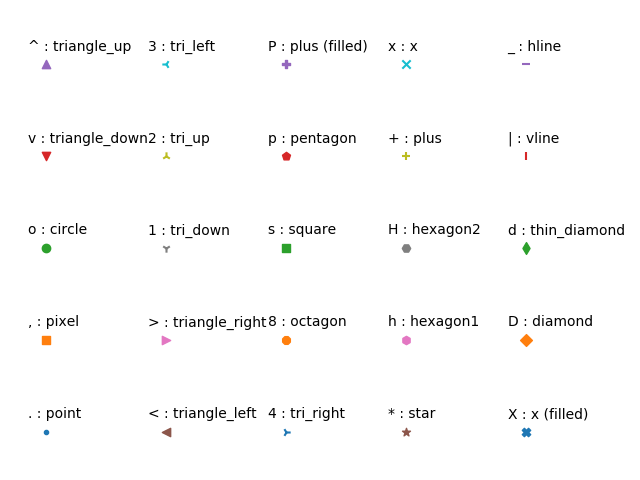
\includegraphics[width=.65\textwidth]{pics/markers.png}
	\caption{Matplotlib中的markers}
	\label{fig:matplotlib-markers}
\end{figure}

\subsubsection{Animation}
Animation可用于制作动画. 初始化函数: 
\begin{python}
	def __init__(self, fig, func, frames=None, init_func=None, fargs=None,
	save_count=None, *, cache_frame_data=True, **kwargs)
	"""
	fig: 绘制动画的地方
	func: 完成动画动作的回调函数. 定义应为: def func(frame, *fargs) -> iterable_of_artists
	frames: 可以认为是每一个动画帧的索引, 通常为iterable对象, frames中的每个值会逐个作为func的第一个参数传入
	init_func: 在绘制第一帧之前调用的函数, 定义应为: def init_func() -> iterable_of_artists
	fargs: 用于func的额外的参数
	repeat_delay: 帧之间的延迟, 单位为毫秒
	repeat: 是否重复播放动画
	blit: 布尔值故,  默认为False. 用于优化绘图, 注意这个参数有点坑, 当其为True时, 会根据artists的zorder来绘图, 当对象没有zorder(如bar)时则会报错
	"""
\end{python}
在使用matplotlib制作动画的过程中, 很重要的是要知道要让什么对象发生变化、发生什么变化 --- 知道了这二者之后就可以在每一帧的更新函数中完成对应的动作了. 

\tbc{red}{注意}: blit参数的使用, 当启用了blit时, 且要对bar改变时, 则会报错: \textit{AttributeError: 'BarContainer' object has no attribute 'get\_zorder'}, 把blit设为False即可. 


\subsubsection{调整子图间距}
\begin{itemize}
	\item plt.tight\_layout()
	\item plt.subplot\_adjust(left=None, bottom=None, right=None, top=None, wspace=None, hspace=None)
\end{itemize}

\subsubsection{显示中文}
\begin{python}
	plt.rcParams['font.sans-serif'] = ['SimHei'] # 步骤一(替换sans-serif字体)  
	plt.rcParams['axes.unicode_minus'] = False  # 步骤二(解决坐标轴负数的负号显示问题)
\end{python}

\subsection{python中的线程有什么问题?怎么解决?}
python 中有一个叫 GIL(Global Interpreter Lock, 全局解释器锁) 的玩意儿, 每个线程想要执行必须先获取到这把锁, 不管你 CPU 有几个核心, 锁只有一把. 所以每次只能有一个线程在执行. 

 
\subsection{生成器}
生成器其实是一种迭代器的一种, 实现了 \mintinline{python}{__iter__, __next__} 方法. 得到一个生成器一般有两种方法: 
\begin{itemize}
	\item 生成器函数. 即在函数中使用 \mintinline{python}{yield} 关键字;
	
	\item 生成器表达式. 即将列表推导中的 \mintinline{python}{[]} 换成 \mintinline{python}{()};
\end{itemize}
 
\subsection{可迭代对象与迭代器}
\textbf{可迭代对象}是实现了 \mintinline{python}{__iter__} 方法的类, 可以通过 \mintinline{python}{for} 循环迭代读取数据元素. 有两类可迭代对象: 
\begin{itemize}
	\item 集合类型的数据结构, \mintinline{python}{list, tuple, dict, set, str} 等;
	
	\item 实现了 \mintinline{python}{__iter__} 方法的类;
\end{itemize}
可迭代对象遍历完一般后还可以继续使用. 

\textbf{迭代器}实现了 \mintinline{python}{__iter__} 和 \mintinline{python}{__next__}. 迭代器遍历完后就空了, 一般会抛出 \mintinline{python}{StopIteration} 异常. 一般可以通过 \mintinline{python}{next} 函数来获取迭代器的下一个元素. 

\subsection{多个装饰器的执行顺序}
当用多个装饰器装饰一个函数时, 装饰器的装饰顺序和执行顺序: 
\begin{itemize}
	\item 装饰顺序是由下至上的, 即解释器执行的顺序(运行时);
	
	\item 调用顺序是自上而下的(调用时);
\end{itemize}
举个例子
\begin{python}
	def AA(func):
		print('AA 1')  # 只会在装饰时执行
		def func_a(*args, **kwargs):
			print('AA 2')  # 每次调用都会执行
			return func(*args, **kwargs)
		return func_a
	
	def BB(func):
		print('BB 1')
		def func_b(*args, **kwargs):
			print('BB 2')
			return func(*args, **kwargs)
		return func_b
	
	@BB
	@AA
	def f(x):
		print('F')
		return x * 10
	
	print(f(1))
	
	# 最终输出
 	# AA 1
	# BB 1
	# BB 2
	# AA 2
	# F
	# 10
\end{python}

对 \mintinline{python}{f} 装饰后相当于\textbf{先进行装饰}, 即 \mintinline{python}{BB(AA(f))}, 即先用 \mintinline{python}{AA} 装饰(因此输出了 \mintinline{python}{AA 1}), 再用 \mintinline{python}{BB} 装饰(因此输出了 \mintinline{python}{BB 1}). \textbf{调用时}, 则等价于 \mintinline{python}{BB(AA(f))(1)}, 因此会调用 \mintinline{python}{func_b(1)}(因此输出了 \mintinline{python}{BB 2}), 再调用 \mintinline{python}{func_a(1)}(因此输出了 \mintinline{python}{AA 2}), 最终调用 \mintinline{python}{f(1)}. 


\subsection{GIL}
Global Interpreter Lock, 全局解释器锁, 是 CPython 解释器的特性. 在一个进程中, 每个线程想要运行都需要先获得 GIL. 因此, 在一个进程内, 一个时刻只能有一个线程在运行, 即使有多个 CPU. 由于 python 的内存管理不是线程安全的, 为了保证多线程之间数据的一致性, GIL 可以防止在同一时刻有多个线程执行字节码. 

一般来说, 一个线程执行了一定数量的字节码, 一定时间或者遇到 IO 任务后会自动释放 GIL, 从而出发线程调度. 

既然一次只能执行一个线程, 那么 python 里的多线程还有必要吗? 虽然有点鸡肋, 但还是有用的. 在 IO 密集型的应用中, 比如线程一直在等待网络响应, 读写磁盘, 等待用户输入等, 这个时候多线程还是能节省时间的.

既然已经有了 GIL, 那就一定线程安全了吗? 并不是. GIL 保证的是每一条字节码在执行过程中的独占性, 即每一条字节码的执行都是原子性的. 但在多个字节码之间, GIL 可能被释放, 则可能会产生多个线程修改临界区的问题. 因此 python 的 \mintinline{python}{multithreading} 模块中还有一个线程锁, 用来对临界区进行加锁.

参考资料: \href{http://cenalulu.github.io/python/gil-in-python/#:~:text=GIL%E5%85%A8%E7%A7%B0Global%20Interpreter%20Lock%E4%B8%BA%E4%BA%86%E9%81%BF%E5%85%8D%E8%AF%AF%E5%AF%BC%EF%BC%8C%E6%88%91%E4%BB%AC%E8%BF%98%E6%98%AF%E6%9D%A5%E7%9C%8B%E4%B8%80%E4%B8%8B%E5%AE%98%E6%96%B9%E7%BB%99%E5%87%BA%E7%9A%84%E8%A7%A3%E9%87%8A%EF%BC%9A%20In%20CPython%2C%20the%20global%20interpreter,mainly%20because%20CPython%E2%80%99s%20memory%20management%20is%20not%20thread-safe.}{Python的GIL是什么鬼,多线程性能究竟如何}.
	
\subsection{python 内存管理}